\documentclass[11pt,a4paper]{report}
\usepackage[utf8]{inputenc}
\usepackage[french]{babel}
\usepackage[T1]{fontenc}
\usepackage{amsmath}
\usepackage{amsfonts}
\usepackage{amssymb}
\usepackage{xcolor}

\usepackage{geometry}
\geometry{hmargin=2.5cm,vmargin=1.5cm}
\usepackage{wasysym}
\usepackage{graphicx}

\author{Mathieu Sarrat}
\title{LP3 - Notion de viscosité d'un fluide. Écoulements visqueux}

\makeatletter
\renewcommand{\thesection}{\@arabic\c@section}
\makeatother


\begin{document}
\maketitle

\section{Introduction}

Imaginons un long récipient cylindrique de rayon $R$ contenant un fluide, le tout étant au repos. 

On commence alors à faire tourner le récipient autour de son axe principal, à vitesse angulaire fixe $\Omega_0$. Dans un premier temps, seul le fluide immédiatement au contact de la paroi cylindrique est entraîné par le mouvement du récipient. Plus on attend, plus le mouvement se propage vers les couches internes du fluide. Si on attend encore, la totalité du fluide finit par tourner à la même vitesse angulaire que le récipient. 

%On a transféré de proche en proche, par diffusion radiale, de la quantité de mouvement. Ce transfert ne saurait être de nature convective, puisque le fluide se déplace de façon tangentielle au rayon d'un cercle centré sur l'axe du cylindre : le transport convectif est donc tangentiel, et non radial, dans cette expérience. Il s'agît en réalité de transport par diffusion, tout comme une goutte d'encre déposée dans un verre d'eau va s'étendre, jusqu'à ce que la concentration en encre dans le verre soit homogène.

Notons qu'à tous les moments de cette expérience, la vitesse du fluide au contact de la paroi est égale à la vitesse de la paroi : il existe ainsi une force de frottement entre les couches fluides au contact de la paroi qui permet l'entrainement de fluide à partir de la paroi. Dans le fluide, la couche la plus rapide entraîne la couche la plus lente, qui gagne donc de l'énergie cinétique. Cette force de frottement est assurée par une propriété du fluide que nous appellerons viscosité.

On peut analyser cette expérience d'une autre manière, ou plutôt "à l'envers" : comme la vitesse de la paroi n'est pas transmise instantanément au cœur du fluide, on peut dire que le fluide résiste à sa mise en mouvement. La viscosité d'un fluide peut donc être considérée comme sa capacité de résistance à l'écoulement : c'est pour cela qu'on a tendance à qualifier de visqueux un liquide plutôt épais (le miel, l'huile), dans la vie quotidienne. Cette résistance aura tendance à ralentir la couche de fluide la plus rapide, et donc à lui faire perdre de l'énergie. 

%Cette énergie perdue est transférée sous deux formes : une énergie cinétique "ordonnée" permettant la mise en mouvement à l'échelle mésoscopique de la couche de fluide voisine (les particules fluides acquièrent une quantité de mouvement moyenne non nulle) et une énergie cinétique "désordonnée", microscopique, sous forme d'agitation thermique (la quantité de mouvement moyenne communiquée à la particule fluide de cette manière est nulle). Une partie de l'énergie est donc dégradée par le frottement visqueux, sous forme de chaleur.
%
%On comprend alors qu'en l'absence de source d'énergie extérieure (maintenir la rotation du cylindre via un moteur, et donc maintenir un apport constant d'énergie cinétique), la couche la plus rapide va être progressivement freinée par la couche la plus lente. Le processus diffusif va essayer d'homogénéiser la quantité de mouvement à l'échelle mésoscopique, mais ce processus est dissipatif (d'où son irréversibilité fondamentale). Il va donc entraîner, progressivement, l'arrêt total du mouvement du fluide.
%
%La viscosité permet la mise en mouvement d'un fluide si on fournit de l'énergie à ce fluide, mais elle n'est en aucun cas capable d'assurer un quelconque mouvement perpétuel.

Quelque soit le point de vue adopté, les diverses couches d'un fluide en mouvement ne peuvent pas glisser librement les unes sur les autres : tout se passe comme s'il y avait des frottements au sein du fluide.

\newpage
\section{La viscosité}\label{sec:1}

\subsection{Définition}\label{sec:1.1}

On suppose un fluide dont le champ de vitesse $\bold{v} = v_z\left(\bold{r},t\right)\bold{e}_z$ est tel que les couches supérieures se déplacent plus vite que les couches inférieures : il y a un gradient de vitesse selon l'axe $x$. De plus, on suppose l'invariance du système par translation selon $y$ et $z$, de sorte que $v_z\left(\bold{r},t\right) = v_z\left(x,t\right)$. Cette approximation est satisfaisante lorsque les dimensions de l'écoulement selon $y$ et $z$ sont grandes vis à vis de l'épaisseur (en $x$) de la couche de fluide (les frontières en $y$ et $z$ sont suffisamment loin de la zone étudiée pour estimer qu'elles n'influent pas sur le comportement du fluide dans cette région).

\begin{figure}[h!]
\begin{center}
	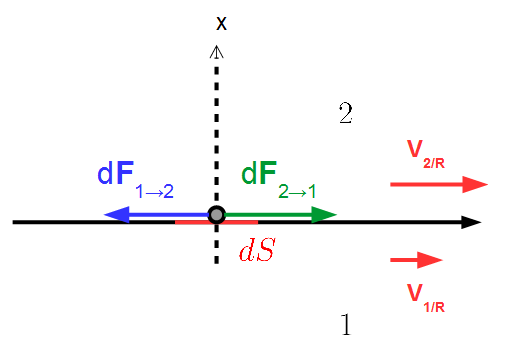
\includegraphics[scale = 0.5]{viscosite_def4.png}
	\caption{Illustration de la définition de la viscosité} 
	\label{fig:transport_1Dmicromodel}
\end{center}
\end{figure}

Considérons maintenant deux éléments de ce fluide notés 1 et 2 et séparés par une surface imaginaire $\mathcal{S}$ parallèle au plan $(yOz)$, positionnée à une côte $x$ quelconque [Figure].

La force $d\bold{F}_{2\rightarrow 1}$ exercée par l'élément 2 (plus rapide) sur l'élément 1 (plus lent) à travers l'élément de surface $d\mathcal{S}$ a deux types de contributions :
\begin{itemize}
	\item une partie normale à $d\mathcal{S}$, $d\bold{F}_{2\rightarrow 1}^n$ : ce sont les contraintes de pression,
	\item une partie tangentielle à $d\mathcal{S}$, $d\bold{F}_{2\rightarrow 1}^t$ : ce sont les contraintes de cisaillement, liées à la viscosité.
\end{itemize}

Laissons de côté la composante normale pour nous consacrer à la force de viscosité. Cette dernière est :
\begin{itemize}
	\item proportionnelle à la surface de contact,
	\item dirigée selon le mouvement relatif de la couche voisine (une couche plus rapide e, la plus lente freine la plus rapide).
\end{itemize}

Pour une catégorie de fluides, qualifiés de newtoniens, la force de viscosité est proportionnelle au gradient de vitesse selon la direction transverse à celle de la force.
Dans l'exemple proposé sur la Figure :
\begin{equation}
	d\bold{F}_{2\rightarrow 1}^t = \eta \frac{\partial v_z}{\partial x} 
	d\mathcal{S}\;\bold{e}_z
	\label{eq:viscosite}
\end{equation}
La grandeur $\eta$ est positive et est appelée \textbf{viscosité dynamique}. Elle est le \textbf{coefficient de proportionnalité} entre la \textbf{force tangentielle} exercée par le fluide extérieur sur la surface du système et le \textbf{gradient du champ des vitesses selon la direction perpendiculaire} à cette surface.

\subsubsection{Viscosité dynamique}
\begin{itemize}
	\item son unité est le Poiseuille (P$\ell$, ou Pa.s dans le système international)
	\item elle dépend fortement de la température en règle générale (diminue avec $T$ pour les liquides, augmente pour les gaz)
	\item elle est peu dépendante de la pression
\end{itemize}

On la mesure avec un viscosimètre.

\subsubsection{Viscosité cinématique}
On définit la \textbf{viscosité cinématique} en divisant $\eta$ par la masse volumique $\rho$ :
\begin{equation}
	\nu \equiv \frac{\eta}{\rho}.
\end{equation}
Son unité est le $\text{m}^2.\text{s}^{-1}$.

\subsubsection{Ordres de grandeur}
Donnons enfin quelques ordres de grandeur pour $\eta$ et $\nu$, à $T = 293$ K.

\begin{center}
\begin{tabular}{|c|c|c|c|c|}
  \hline
  Corps & Air & Eau & Huile d'olive & Glycérine\\
  \hline
  $\eta$ ($\text{Pa.s}$) & $\sim 10^{-5}$ & $\sim 10^{-3}$ & $\sim 0.1$ & $\sim 1.5$\\
  \hline
  $\nu$ ($\text{m}^2\text{s}^{-1}$) & $\sim 10^{-5}$ & $\sim 10^{-6}$ & $\sim 10^{-4}$ & $\sim 10^{-3}$ \\
  \hline
\end{tabular}
\end{center}

\subsubsection{Opposition des actions réciproques (Troisième Loi de Newton)} 

Par opposition des actions réciproques, $d\bold{F}_{2\rightarrow 1} = - d\bold{F}_{1\rightarrow 2}$ :
\begin{equation}
	d\bold{F}_{1\rightarrow 2} = - \eta \frac{\partial v_z}{\partial x} d\mathcal{S}\;\bold{e}_z.
\end{equation}

Comme $\partial v_z/\partial x > 0$, on a bien $d\bold{F}_{1\rightarrow 2}$ dirigée selon $-\bold{e}_z$ : si on se place dans un référentiel où 2 est fixe, l'élément 1 se déplace bien selon $-x$.

On retiendra que lors du frottement en deux couches de fluide : 
\begin{itemize}
	\item la couche la plus lente est accélérée/entraînée par la plus rapide, 
	\item la plus rapide est freinée par la couche la plus lente.
\end{itemize}


\subsubsection{Force volumique de viscosité}

Considérons maintenant un petit volume cubique $d\mathcal{V} = dxdydz$ de fluide [Figure] et un gradient de vitesse $v_z$ vertical (selon $x$).
Placé dans l'écoulement uni-dimensionnel précédent $\bold{v} = v_z\left(x,t\right)\bold{e}_z$, les seules forces de viscosité qui vont s'exercer sur lui seront celles s'exerçant sur les surfaces $d\mathcal{S}_x = dy dz$ de côtes respectives $x$ et $x+dx$ selon l'axe $x$. Ces forces s'écrivent :
\begin{itemize}
	\item pour la surface de côte $x+dx$,
	\begin{equation}
		d\bold{F}_{\text{haut}\rightarrow d\mathcal{V}}^t =  \eta \left(\frac{\partial v_z}{\partial x}\right)_{x+dx} d\mathcal{S}_x\;\bold{e}_z,
	\end{equation}
	\item et pour la surface de côte $x$,
	\begin{equation}
		d\bold{F}_{\text{bas}\rightarrow d\mathcal{V}}^t = - \eta \left(\frac{\partial v_z}{\partial x}\right)_{x}    d\mathcal{S}_x\;\bold{e}_z.
	\end{equation}
\end{itemize}

La force résultante $d\bold{F}^t = d\bold{F}_{\text{haut}\rightarrow d\mathcal{V}}^t + d\bold{F}_{\text{bas}\rightarrow d\mathcal{V}}^t$ s'écrit :
\begin{equation}
	d\bold{F}^t = \eta d\mathcal{S}_x \left[ -\left(\frac{\partial v_z}{\partial x}\right)_{x}
	+ \left(\frac{\partial v_z}{\partial x}\right)_{x+dx}  \right]\;\bold{e}_z,
\end{equation}

Comme $d\mathcal{V} = dx d\mathcal{S}_x$, en utilisant la définition de la dérivée partielle seconde par rapport à $x$ on obtient
\begin{equation}
	\bold{F}^t = \eta \frac{\partial^2 v_z}{\partial x} d\mathcal{V}\;\bold{e}_z.
\end{equation}

La force de viscosité par unité de volume s'écrit donc
\begin{equation}
	{\bold{f}_v}^t = \frac{\partial^2 v_z}{\partial x^2}.
\end{equation} 

Pour un écoulement tridimensionnel incompressible, on doit ajouter les forces exercées sur les autres surfaces du cube. On peut montrer que ${\bold{f}_v}^t$ devient 
\begin{equation}
	{\bold{f}_v}^t = \eta\Delta \bold{v},
\end{equation}
où $\Delta$ désigne l'opérateur Laplacien :
\begin{equation}
	\Delta\bold{v} = \Delta v_x \bold{e}_x + \Delta v_y \bold{e}_y + \Delta v_z \bold{e}_z.
\end{equation}

\begin{figure}[h!]
\begin{center}
	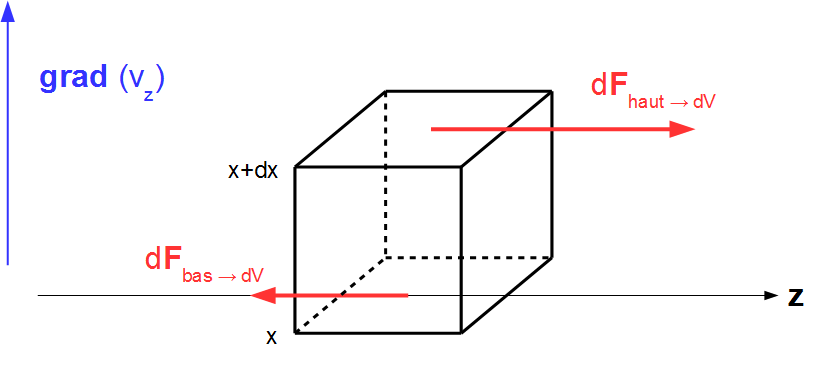
\includegraphics[scale = 0.5]{visco_vol.png}
	\caption{Calcul de la force volumique de viscosité s'exerçant sur le volume $d\mathcal{V}$} 
	\label{fig:visco_vol}
\end{center}
\end{figure}

\subsubsection{Remarque 1 :}
Cette force volumique n'est qu'un équivalent mathématique bien pratique (la résultante de plusieurs forces), car ces forces s'exercent bien sur une surface.

\subsubsection{Remarque 2 :}
Cette expression n'est valable que pour un écoulement incompressible (on peut vérifier que l'écoulement test sur lequel nous nous basons l'est), caractérisé par $\text{div}\bold{v} = 0$. Si l'écoulement n'est pas incompressible, le terme supplémentaire
\begin{equation}
	\left(\zeta + \frac{\eta}{3} \right)\textbf{grad}\;\left(div\bold{v}\right)
\end{equation}
doit être ajouté à la force de viscosité. La grandeur $\zeta$ est appelée \textbf{seconde viscosité} ou \textbf{viscosité de volume}.

Dans toute la suite, \textbf{on ne considèrera que des écoulements incompressibles}, de sorte que ce terme supplémentaire n'apparaîtra jamais dans les calculs. Cette hypothèse est valable pour les liquides et les gaz tant que la vitesse caractéristique de l'écoulement est bien inférieure à celle de propagation du son dans le fluide.

\subsection{Transport diffusif de la quantité de mouvement}\label{sec:1.2}

L'équilibre thermodynamique est perturbé par la mise en mouvement d'une partie du milieu. L'apparition d'un gradient de vitesse (un écart à l'équilibre) est le moteur d'un phénomène de transport dont le but est la "relaxation" de cet écart. Nous avons vu que les forces de viscosité freinaient les couches les plus rapides du fluide tout en accélérant les couches les plus lentes. 

Reprenons l'expérience avec laquelle nous avons démarré cette leçon : la rotation du cylindre extérieur provoque une mise en mouvement progressive du fluide, jusqu'au point où tout le fluide tourne avec la même vitesse angulaire que le récipient. On a transféré de proche en proche de la quantité de mouvement, depuis la source jusqu'à travers tout le fluide. Ce transfert ne saurait être de nature convective, puisque le fluide se déplace de façon tangentielle au rayon d'un cercle centré sur l'axe du cylindre : le transport convectif est donc tangentiel et non radial dans ce cas. Le transport impliqué dans cette expérience est un transport par diffusion, tout comme une goutte d'encre déposée dans un verre d'eau va s'étendre jusqu'à ce que la concentration en encre dans le verre soit homogène.

Si on applique le principe fondamental de la dynamique à l'élément de volume $\mathcal{V}$, que l'on imagine soumis uniquement aux forces de viscosité définies plus haut on obtient immédiatement une équation de diffusion :
\begin{equation}
	\rho\frac{\partial \bold{v}}{\partial t} = \eta \Delta\bold{v},
\end{equation}
et, en divisant par $\rho$,
\begin{equation}
	\frac{\partial \bold{v}}{\partial t} = \nu \Delta\bold{v}.
\end{equation}

Cette équation décrit la diffusion du champ des vitesses $\bold{v}$, où la viscosité cinématique joue le rôle de coefficient de diffusion, comme on pouvait s'y attendre du fait de la dimension de $\nu$ ($\text{Longueur}^2/\text{Temps}$). 

En régiment laminaire, et en négligeant le poids et les forces de pression, l'équation de Navier-Stokes se ramène à une "simple" équation de diffusion du champ des vitesses :
\begin{equation}
	\frac{\partial \bold{v}}{\partial t} = \nu \Delta \bold{v},
\end{equation}
où la viscosité cinématique joue le rôle de coefficient de diffusion.

\subsubsection{Remarque 1 : vitesse ou quantité de mouvement ?}
Puisque nous supposons un écoulement incompressible, la masse volumique du fluide est une constante qu'il est possible de faire entrer dans les dérivées.
En remarquant que la quantité $\rho \bold{v}$ est une quantité de mouvement par unité de volume, on obtient bien une équation de diffusion de la quantité de mouvement.

\subsubsection{Remarque 2 : compétition entre transport convectif et transport diffusif}
Lorsque le transport convectif de la quantité de mouvement n'est pas négligeable, il masque totalement le transport par diffusion lié à la viscosité. 

\subsubsection{Remarque 3 : interprétation microscopique}

Il est possible d'interpréter de façon microscopique le phénomène de viscosité de la même manière que celui de diffusion de la chaleur ou de la matière. 
Reprenons le modèle uni-dimensionnel utilisé pour définir la viscosité en 2.1.

D'un point de vue macroscopique et pour un fluide newtonien, on définit la densité volumique de flux de quantité de mouvement comme :
\begin{equation}
	\bold{J}_\bold{p} = - \eta\frac{\partial v_z}{\partial x}\bold{e}_x.
\end{equation}

On peut montrer avec un modèle uni-dimensionnel relativement simple (cf. leçon sur les phénomènes de transport) que
\begin{equation}
	\bold{J}_\bold{p} = - \rho\frac{\ell v_m}{3}\frac{\partial v_z}{\partial x}\bold{e}_x = -\eta \frac{\partial v_z}{\partial x}\bold{e}_x.
\end{equation}
où $\ell$ désigne le libre parcours moyen d'une molécule (distance moyenne entre deux collisions), $v_m$ sa vitesse moyenne et $\rho$ la masse volumique.

Il en découle que 
\begin{equation}
	\eta = \rho \frac{\ell}{3}v_m \propto \frac{\left(mT\right)^{1/2}}{R^2},
\end{equation}
avec $m$ la masse d'une molécule, $R$ son rayon et $T$ la température du fluide. 
On constate l'augmentation de la viscosité avec la température pour un fluide incompressible.\\

Ce modèle ne fonctionne pas pour les liquides du fait des interactions de Van der Waals, négligeables pour des gaz suffisamment dilués, mais jouant un rôle majeur dans les liquides. L'agitation thermique nuit à l'ordre créé par ces interactions, provoquant une diminution de la viscosité lorsque $T$ augmente dans un liquide.

\subsection{Fluides newtoniens et non-newtoniens}

Nous avons défini les fluides newtoniens comme ceux pour lesquels la relation de proportionnalité entre la contrainte tangentielle et le gradient de vitesse est vérifiée expérimentalement (cf. équation \eqref{eq:viscosite}).

Lorsqu'il n'y a \textbf{plus proportionnalité} entre la contrainte exercée et le gradient de vitesse on parle de \textbf{fluide non-newtonien}. 
Leur étude est l'objet de la \textbf{rhéologie}. Les fluides non-newtoniens sont très répandus : sang, boue, mayonnaise, yaourt, dentifrice, peinture, pour n'en citer que quelques uns. Ces propriétés particulières s'expliquent par la présence d'objets de grande taille par rapport à l'échelle atomique, mais petits devant les dimensions caractéristiques de l'écoulement.

Donnons quelques exemples, sans prétendre être exhaustifs. On parle de fluide rhéo-fluidifiant lorsque la viscosité diminue alors que la contrainte exercée devient plus forte : c'est notamment le cas du shampooing ou des crèmes cosmétiques. Un fluide est au contraire, rhéo-épaississant lorsque sa viscosité augmente avec la contrainte appliquée, c'est le cas du sable mouillé ou du mélange eau-maïzena. Le yaourt, le magma, les boues, la mayonnaise ou encore le dentifrice sont des fluides non-newtoniens.\\

Nous ne considèrerons dans cette leçon que des fluides newtoniens.

\newpage
\section{Dynamique des fluides incompressibles visqueux}\label{sec:2}

\subsection{Équation de Navier-Stokes}\label{sec:2.1}

\begin{itemize}
	\item La prise en compte des forces de viscosité dans le bilan des forces agissant sur une particule fluide conduit à l'équation de Navier-Stokes.\\
	
	\item \textcolor{red}{Inventaire des forces agissant sur particule fluide de masse $\rho d\mathcal{V}$ :}
	\begin{itemize}
		\item forces de pression (résultante des contraintes normales)
		\item forces de viscosité (résultante des contraintes tangentielles)
		\item pesanteur (champ de gravitation $\bold{g}$). 
	\end{itemize}
	
	\item \textcolor{red}{PFD pour la particule fluide :}
	\begin{equation}
		\rho\frac{d\bold{v}}{dt} = \rho\bold{g} - \bold{\text{grad}}\;(p) + \eta\Delta\bold{v},
	\end{equation}
	
	Développer l'expression de la dérivée totale $d\bold{v}/dt$
	\begin{equation}
		\rho\left(\frac{\partial\bold{v}}{\partial t}+\left(\bold{v}\cdot\bold{\text{grad}}\right)\bold{v}\right)=\rho\bold{g}-\bold{\text{grad}}(p)+\eta\Delta\bold{v},
	\end{equation}	
	
	Diviser par $\rho$ pour faire apparaître la \textbf{viscosité cinématique}
	\begin{equation}
		\frac{\partial\bold{v}}{\partial t} + \left(\bold{v}\cdot\bold{\text{grad}}\right)\bold{v} = \bold{g} - \frac{1}{\rho}\bold{\text{grad}}(p) + \nu\Delta\bold{v}.
	\end{equation}
\end{itemize}

\subsubsection{Remarque 1 : validité}
N.S. n'est vraie que si :
\begin{itemize}
	\item fluide newtonien : la viscosité sera supposée constante
	\item écoulement incompressible : $\text{div}\bold{v} = 0$, $\rho$ constante.\\
\end{itemize}

\subsubsection{Remarque 2 : bilan de quantité de mouvement et lien avec \ref{sec:1.2}}
\begin{itemize}
	\item Navier-Stokes $=$ bilan local de quantité de mouvement pour fluide visqueux incompressible
	\item Sans forces de pression, viscosité, poids : N-S devient
	\begin{equation}
		\frac{\partial\bold{v}}{\partial t} + \left(\bold{v}\cdot\bold{\text{grad}}\right)\bold{v}= 0
	\end{equation}
	Conservation de la quantité de mouvement lors de l'écoulement. Transport convectif.
\end{itemize}

\subsubsection{Remarque 3 : terme d'advection}
\begin{itemize}
	\item En $v^2$, donc non-linéaire, complique la résolution de l'équation.\\
\end{itemize}

\subsubsection{Remarque 4 : conditions aux limites sur le champ des vitesses}
\begin{itemize}
	\item Résolution d'une équation différentielle : conditions aux limites nécessaires.
	\item Limitation au cas d'un contact avec un solide : à l'interface \textcolor{red}{$\bold{v}_{solide} = \bold{v}_{fluide}$}\\
\end{itemize}

\textcolor{red}{Explication :}
\begin{itemize}
	\item paroi imperméable : \textcolor{blue}{égalité des composantes normales} 
	\item viscosité : \textcolor{blue}{égalité des composantes tangentielles}
\end{itemize}

\subsubsection{Remarque 5 : besoin d'approximations}
\begin{itemize}
	\item Résolution analytique délicate ou impossible sans approximation $\Rightarrow$ Exemple avec Nombre de Reynolds.
\end{itemize}

\subsection{Nombre de Reynolds et régimes d'écoulement}\label{sec:2.2}

\begin{itemize}
	\item Généralement : convection et diffusion coexistent;
	\item La géométrie et la vitesse de l'écoulement favorisent l'un ou l'autre;
	\item Nombre de Reynolds $Re$ : comparer le terme d'advection $\rho\left(\bold{v}.\textbf{\text{grad}}\right)\bold{v}$ au terme de viscosité $\nu\Delta\bold{v}$;
\end{itemize} 

\textcolor{red}{Par analyse dimensionnelle $\Rightarrow$ définition de $Re$ :}
\begin{equation}
	\frac{|\rho\left(\bold{v}.\textbf{\text{grad}}\right)\bold{v}|}{|\nu\Delta\bold{v}|} = \frac{\rho U^2/L}{\eta U/L^2} = \frac{UL}{\nu} \equiv Re,
\end{equation}
$U$ et $L$ vitesse et longueur caractéristiques du problème.

\textcolor{red}{Interprétation de $Re$ :}
\begin{itemize}
\item comparaison des flux de quantité de mouvement associés aux transport convectif et diffusif :
	\begin{equation}
		Re \simeq \frac{\text{flux convectif}}{\text{flux diffusif}}
	\end{equation}
\item comparaison des temps caractéristiques de transport sur une longueur de l'ordre de $L$ :
	\begin{equation}
		Re = \frac{\tau_\text{diffusion}}{\tau_\text{convection}}.
	\end{equation}
	Le mécanisme le plus rapide (petit $\tau$) domine.
\end{itemize}

\textcolor{red}{Cas limites :}
\begin{itemize}
	\item\textbf{faible Reynolds} : écoulement rampant, domination de la viscosité et du transport diffusif, écoulements stables, cohésion importante entre les couches de fluide.
	Observable à faible vitesse, systèmes de petite taille, fluides très visqueux.
	\item\textbf{fort Reynolds} : domination de la convection, grande non-linéarité (terme en $\rho\left(\bold{v}.\textbf{\text{grad}}\right)\bold{v}$), peu stable (instabilités, peut conduire à un écoulement turbulent (formation de tourbillons de taille variable)). 
	Cas des écoulements à vitesse élevée sur systèmes de grande taille ou peu visqueux.
\end{itemize}

\textcolor{red}{Cas particulier : écoulement laminaire} (ou parallèle)
\begin{itemize}
	\item Même à grand Reynolds ($Re < 2000$), la diffusion peut dominer si l'écoulement est laminaire, du fait d'une géométrie particulière. 
	Les tranches (lames) de fluide glissent les unes par rapport aux autres, sans se mélanger, se croiser, se déstructurer.
	\item Exemple : le cylindre de l'intro. La convection ne peut pas se faire radialement, donc c'est la diffusion qui transporte radialement, faute de mieux.
	Attention, si localement une vitesse radiale apparaît, la convection peut reprendre le dessus (instabilité puis turbulence)
\end{itemize}

\subsection{Aspect énergétique}\label{sec:2.3}

Prenons l'équation de Navier-Stokes et utilisons l'égalité mathématique suivante :
\begin{equation}
	\left(\bold{v}\cdot\textbf{grad}\right)\bold{v} = \frac{1}{2}\textbf{grad}\;v^2 + \textbf{rot}\;\bold{v}\times\bold{v}.
\end{equation}

On obtient
\begin{equation}
	\frac{\partial\bold{v}}{\partial t} +  \textbf{grad}\left(\frac{v^2}{2}\right) + \textbf{rot}\;\bold{v}\times\bold{v}
	= - \frac{1}{\rho}\textbf{grad}\;p + \bold{g} + \nu\Delta\bold{v}.
\end{equation}

L'équation de Navier-Stokes fait intervenir des forces par unité de volume. On s'intéresse à l'aspect énergétique du problème : multiplions donc par un déplacement élémentaire $d\bold{r} = \bold{v}dt$. On trouve
\begin{equation}
	\frac{\partial\bold{v}}{\partial t}\cdot d\bold{r} + \textbf{grad}\left(\frac{v^2}{2}\right)\cdot d\bold{r} = - \frac{1}{\rho}\textbf{grad}\;(p) \cdot d\bold{r}
	+ \bold{g}\cdot d\bold{r} + \nu\Delta\bold{v}\cdot d\bold{r}
\end{equation}
comme $\left(\textbf{rot}\;\bold{v}\times\bold{v}\right)\cdot\bold{v} = 0$. 

Supposons un écoulement stationnaire $\partial \bold{v}/\partial t$ et incompressible $\rho = cte$ :
\begin{equation}
	\textbf{grad}\left(\frac{v^2}{2} + \frac{p}{\rho} \right)\cdot d\bold{r} = \bold{g}\cdot d\bold{r} +  \nu\Delta\bold{v}\cdot \bold{v}dt
\end{equation}
Or, $\bold{g}$ étant supposé uniforme,
\begin{equation}
	\bold{g}\cdot d\bold{r} = d\left(\bold{g}\cdot\bold{r}\right)
\end{equation}
et comme $\bold{v}$ et $p$ ne dépendent que de $\bold{r}$ (régime stationnaire), le premier terme est une différentielle totale
\begin{equation}
	\textbf{grad}\left(\frac{v^2}{2} + \frac{p}{\rho} \right)\cdot d\bold{r} = d\left(\frac{v^2}{2} + \frac{p}{\rho}\right),
\end{equation}
d'où,
\begin{equation}
	d\left(\frac{v^2}{2} + \frac{p}{\rho} - \bold{g}\cdot\bold{r}\right) =  \nu\Delta\bold{v}\cdot \bold{v}dt.
\end{equation}

On reconnaît là une version fluide du théorème de l'énergie mécanique : 
\begin{itemize}
	\item $\frac{\bold{v}^2}{2}$ est l'énergie cinétique par unité de masse d'une particule fluide de vitesse $\bold{v}$,
	\item $\frac{p}{\rho}$ est l'énergie potentielle massique associée aux forces de pression, 
	\item $- \bold{g}\cdot\bold{r}$ est l'énergie potentielle de pesanteur (par unité de masse) d'une particule fluide au point $\bold{r}$  
\end{itemize}

Le terme de gauche correspond donc à l'énergie mécanique par unité de masse (énergie massique) du fluide. La variation de cette énergie est égale au travail des forces non-conservatives, comme les forces de frottement visqueux. On peut réécrire cette équation en termes de puissance :

\begin{equation}
	\frac{d}{dt}\left(\frac{v^2}{2} + \frac{p}{\rho} - \bold{g}\cdot\bold{r}\right) =  \nu\Delta\bold{v}\cdot \bold{v}.
\end{equation}

Cette dernière équation permet de traduire le caractère dissipatif des forces de viscosité : l'énergie mécanique d'un fluide qui ne reçoit pas de travail extérieur ne se conserve pas mais diminue à cause des forces de viscosité.

L'énergie perdue par une couche de fluide lors de son frottement avec une couche voisine est transférée sous deux formes : une énergie cinétique "ordonnée" permettant la mise en mouvement à l'échelle mésoscopique de la couche de fluide voisine (les particules fluides acquièrent une quantité de mouvement moyenne non nulle) et une énergie cinétique "désordonnée", microscopique, sous forme d'agitation thermique (la quantité de mouvement moyenne communiquée à la particule fluide de cette manière est nulle). Une partie de l'énergie est donc dégradée par le frottement visqueux, sous forme de chaleur.

On comprend alors qu'en l'absence de source d'énergie extérieure (maintenir la rotation du cylindre via un moteur, et donc maintenir un apport constant d'énergie cinétique), la couche la plus rapide va être progressivement freinée par la couche la plus lente. Le processus diffusif va essayer d'homogénéiser la quantité de mouvement à l'échelle mésoscopique, mais ce processus est dissipatif (d'où son irréversibilité fondamentale). Il va donc entraîner, progressivement, l'arrêt total du mouvement du fluide.

La viscosité permet la mise en mouvement d'un fluide si on fournit de l'énergie à ce fluide, mais elle n'est en aucun cas capable d'assurer un mouvement perpétuel.


\newpage
\section{Écoulements de fluides visqueux}\label{sec:3}

Quelques exemples et une manip.

\subsection{Chute d'une bille dans un fluide visqueux}\label{sec:3.1}

\begin{figure}[h!]
\begin{center}
	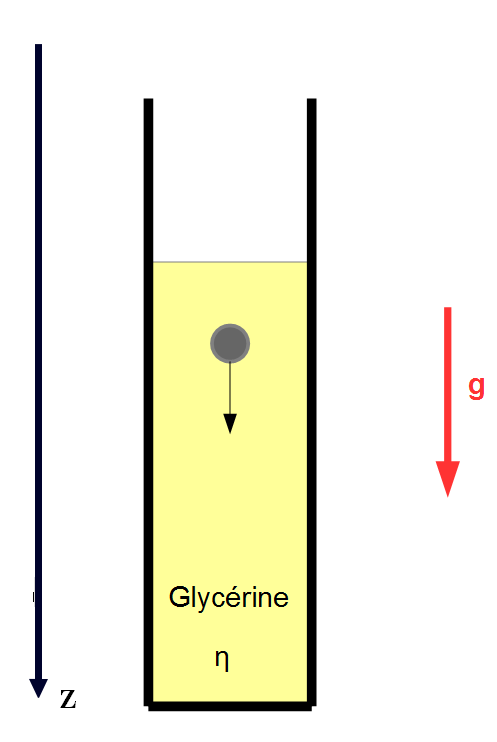
\includegraphics[scale = 0.3]{chute_visco.png}
	\caption{Chute d'une bille dans de la glycérine.} 
	\label{fig:chute_visco}
\end{center}
\end{figure}

\begin{itemize}
	\item Film de la chute d'une bille d'acier (volume $V_b$, masse vol. $\rho_a$, rayon $R$) dans une éprouvette remplie de glycérine (masse vol. $\rho_g$. Acquisition vidéo. Analyse avec Régressi.
	\item Chute sans vitesse initiale.
	\item Tracer $v = f(t)$ : régime transitoire, régime permanent. La vitesse limite permet de mesurer la viscosité.\\
	
	\item \textcolor{red}{Inventaire des forces :}
		\begin{itemize}
			\item Poids : $\bold{P} = \rho_{\text{a}}V_{\text{b}}\bold{g} = \rho_{\text{a}}V_{\text{b}}g\;\bold{e}_z$,
			\item Poussée d'Archimède : $\bold{A} = - \rho_{\text{g}}V_{\text{b}}\bold{g} = - \rho_{\text{g}}V_{\text{b}}g\;\bold{e}_z$,
			\item Frottement visqueux (formule de Stokes) : $\bold{f} = -\alpha\bold{v} = -6\pi\eta R v_{z}\;\bold{e}_z$ (\textcolor{red}{hyp. faible nombre de Reynolds}).
			C'est l'expression de la force de traînée exercée par le fluide sur un objet sphérique en mouvement, à faible nombre de Reynolds. 
			A fort nombre de Reynolds, cette force de frottement est proportionnelle au carré de la vitesse.
		\end{itemize}
		Remarque : formule de Stokes valable jusqu'à $Re \sim 1$ expérimentalement. Penser à vérifier la valeur de $Re$.\\
			
	\item \textcolor{red}{Deuxième Loi de Newton :}
	\begin{equation}
		\rho_a V_b \frac{dv_z}{dt} = \left(\rho_a-\rho_g\right)V_bg -6\pi\eta R v_z,
	\end{equation}
	\begin{equation}
		\frac{dv_z}{dt} + \frac{6\pi\eta R}{\rho_a V_b}v_z = \frac{\rho_a-\rho_g}{\rho_a}g
	\end{equation}
	En régime stationnaire, $dv_z/dt = 0$,
	\begin{equation}
		v_{z,lim} = \frac{2}{9}\frac{g R^2}{\eta}\left(\rho_a-\rho_g\right)
	\end{equation}
	A.N. $R = 1mm$, $\rho_a = 2.5\times 10^{3}kg/m^3$, $\rho_g = 10^3 kg/m^3$, $\eta = 1 Pa.s$. On trouve $v_{z,lim} = 10^{-3}m/s$ d'où $Re \sim 10^-3$.
\end{itemize}

\newpage
\subsection{Écoulement de Couette plan (sans doute pas le temps)}\label{sec:3.2}

Couche de fluide visqueux d'épaisseur $L$ entre deux plaques de surface $\mathcal{S}$. Celle du haut bouge à vitesse $U \bold{e}_z$, celle du bas est fixe.

\begin{figure}[h!]
\begin{center}
	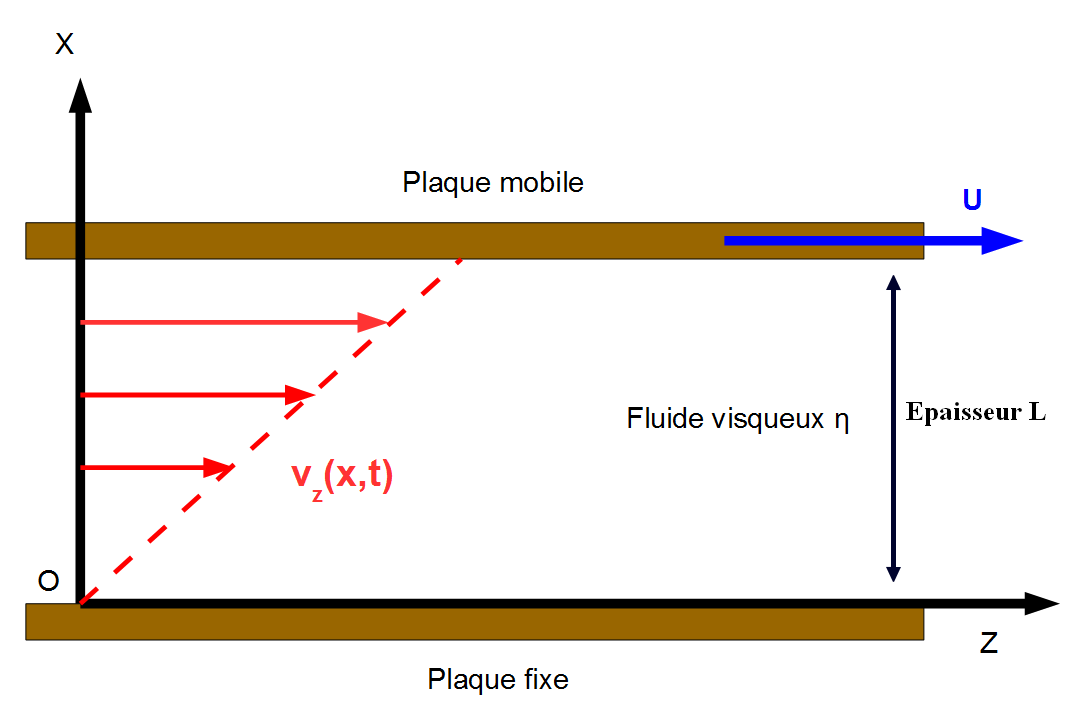
\includegraphics[scale = 0.3]{couette_plan.png}
	\caption{\'Ecoulement de Couette plan} 
	\label{fig:couette_plan}
\end{center}
\end{figure}

\subsubsection{Résolution en régime stationnaire}

\textcolor{red}{Hypothèses :}
\begin{itemize}
	\item Régime stationnaire $\frac{\partial \bold{v}}{\partial t} = 0$
	\item \'Ecoulement uni-directionnel : $\bold{v} = v_z \bold{e}_z$
	\item Invariance par translation selon $y$ et $z$, donc $\bold{v} = v_z(x) \bold{e}_z$ et $p = p(x)$.
	\item Fluide newtonien incompressible\\
\end{itemize}

\textcolor{red}{Terme convectif :}
\begin{equation}
	\left(\bold{v}\cdot\bold{\text{grad}}\right)\bold{v} = v_x\frac{\partial \bold{v}}{\partial x} = 0
\end{equation}
car pas de vitesse selon $x$.\\

\textcolor{red}{Terme diffusif :}
\begin{equation}
	\Delta\bold{v} = \Delta\left(v_z\bold{e}_z\right) = \Delta v_z \bold{e}_z = \frac{\partial^2 v_z}{\partial x^2}\\
\end{equation}

\textcolor{red}{Projection NS selon x :}
\begin{equation}
	0 = -g - \frac{1}{\rho}\frac{\partial p}{\partial x}\\
\end{equation}

\textcolor{red}{Projection NS selon z :}
\begin{equation}
	0 = \nu \Delta v_z = \nu \frac{\partial^2 v_z}{\partial x^2}\\
\end{equation}

\textcolor{red}{Calcul du champ de pression :}
\begin{equation}
	\rho g = - \frac{\partial p}{\partial x} = - \frac{dp}{dp}
\end{equation}
d'où
\begin{equation}
	p = -\rho g x + \text{cte}.
\end{equation}

La pesanteur crée un gradient de pression hydrostatique vertical, qui n'a aucune influence sur l'écoulement.

\textcolor{red}{Calcul du champ des vitesses :}
\begin{equation}
	0 = \frac{\partial v_z^2}{\partial x^2}
\end{equation}
d'où 
\begin{equation}
	v_z(x) = Ax + B
\end{equation}
On détermine $A$ et $B$ avec les conditions de bord : $v_z(0) = 0$ et $v_z(L) = U$.

D'où
\begin{equation}
	v_z(x) = \frac{U}{L}x.
\end{equation}

\subsubsection{Force exercée sur la place pour qu'elle atteigne la vitesse U}

La force exercée par le fluide sur la plaque est une force de viscosité. Sur un élément de surface $d\mathcal{S}$ elle vaut :
\begin{equation}
	d\bold{F}_{\text{flu}\rightarrow\text{plaque}}^t 
	= - \eta \left(\frac{\partial v_z}{\partial x}\right)_{x=L} d\mathcal{S} \bold{e}_z 
	= - \eta \frac{U}{L} d\mathcal{S} \bold{e}_z 
	= - d\bold{F}_{\text{plaque}\rightarrow\text{flu}}^t
\end{equation}
Force totale exercée par la plaque sur le fluide pour maintenir le régime stationnaire (et donc pour maintenir le mouvement de la plaque) :
\begin{equation}
	\bold{F}_{\text{plaque}\rightarrow\text{flu}}^t = \eta \frac{U\mathcal{S}}{L} \bold{e}_z 
\end{equation}

\subsubsection{Dissipation d'énergie}

La plaque inférieure n'est pas entraînée par le fluide, ce qui implique que l'énergie fournie par le mouvement de la plaque supérieure est dissipée au sein du fluide.

\newpage
\subsection{Écoulement de Poiseuille en coordonnées cylindriques (pas le temps)}\label{sec:3.3}

Soit une conduite cylindrique horizontale de diamètre $D$ (rayon $R$, section $\mathcal{S}$) et de longueur $L$, centrée sur l'axe $z$. On applique une différence de pression aux deux extrémités de la conduite, de sorte que $p(z=0) = p_1$ et $p(z=L) = p_2$. Un fluide de viscosité $\eta$ circule dans cette conduite. On décrit le problème en coordonnées cylindriques. 

\begin{figure}[h!]
\begin{center}
	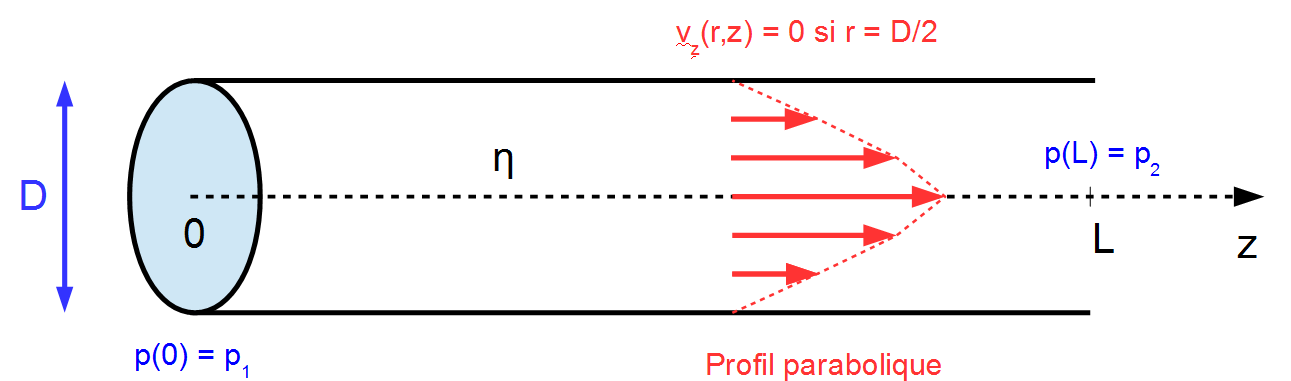
\includegraphics[scale = 0.3]{poiseuille_cyl.png}
	\caption{\'Ecoulement de Poiseuille cylindrique} 
	\label{fig:poiseuille_cyl}
\end{center}
\end{figure}

\subsubsection{Résolution en régime stationnaire}

\textcolor{red}{Hypothèses :}
\begin{itemize}
	\item Régime stationnaire $\frac{\partial \bold{v}}{\partial t} = 0$
	\item \'Ecoulement uni-directionnel : $\bold{v} = v_z \bold{e}_z$
	\item Invariance par rotation d'angle $\theta$ donc $\bold{v} = v_z(r,z) \bold{e}_z$ et $p = p(r,z)$.
	\item Fluide newtonien incompressible\\
	\item Pesanteur négligée (conduite horizontale de faible diamètre)\\ 
\end{itemize}

\textcolor{red}{Condition d'incompressibilité :}
\begin{equation}
	\text{div}\;\bold{v} = \frac{\partial v_z}{\partial z} = 0
\end{equation}
d'où $v_z(r,z) = v_z(r)$. La seule dépendance du champ des vitesses est radiale, $\partial v_z/\partial r = dv_z/dr$.\\

\textcolor{red}{Terme convectif :}
$v_r = 0$ et $\partial v_z/\partial z = 0$ donc terme convectif nul.\\

\textcolor{red}{Terme diffusif :}
\begin{equation}
	\Delta \bold{v} = \Delta v_z \bold{e}_z = \frac{1}{r}\frac{\partial}{\partial r}\left(r \frac{\partial v_z}{\partial r}\right) \bold{e}_z\\
\end{equation}

\textcolor{red}{\'Equation à résoudre :} N.S devient
\begin{equation}
	\textbf{grad}\;p = \eta \Delta \bold{v}
\end{equation}
Pas de composante selon $\bold{e}_{\theta}$.\\


\textcolor{red}{Projection selon $r$ : tuer la dépendance supposée en $r$ de $p$}
\begin{equation}
	\frac{\partial p}{\partial r} = 0
\end{equation}
d'où $p(r,z) = p(z)$ (seule utilité de cette équation), d'où $\partial p/\partial z = dp/dz$.\\

\textcolor{red}{Projection selon $z$}
\begin{equation}
	\frac{dp}{dz} = \eta \frac{1}{r}\frac{d}{d r}\left(r \frac{d v_z}{d r}\right),
\end{equation}
d'où
\begin{equation}
	f(z) = \eta g(r) \equiv K = \text{Cte}.\\
\end{equation}

\textcolor{red}{On commence par résoudre $f(z) = K$ :}
\begin{equation}
	p(z) = Kz + A
\end{equation}
On détermine $K$ et $A$ avec les conditions de bord pour $p$, \textcolor{red}{$p(z) = \frac{p_2 - p_1}{L}z + p_1$}.\\

\textcolor{red}{On détermine $v_z(r)$ :}
\begin{equation}
	\frac{p_2 - p_1}{\eta L} = \frac{1}{r}\frac{d}{d r}\left(r \frac{d v_z}{d r}\right)
\end{equation}
d'où :
\begin{equation}
	r\frac{dv_z}{dr} = \frac{p_2-p_1}{\eta L} \frac{r^2}{2} + \text{B}
\end{equation}
or $B = 0$ car l'équation est vraie en $r = 0$ et que $dv_z/dr$ a une valeur finie en $r = 0$.
\begin{equation}
	v_z(r) = \frac{p_2-p_1}{\eta L}\frac{r^2}{4} + \text{C} = \frac{p_1-p_2}{4\eta L}\left(R^2 - r^2\right)
\end{equation}
où on a utilisé la CL suivante : paroi fixe, donc $v_z (r=R) = 0$.

\subsubsection{Débit-masse et débit-volume}

En régime stationnaire :
\begin{itemize}
	\item \textcolor{red}{Calcul du débit-masse $q_m$}
	\begin{equation}
		q_m = \iint_\mathcal{S} \rho v_z d\mathcal{S} = \iint_\mathcal{S}\rho v_z rdrd\theta = 2\pi\rho\frac{p_1-p_2}{4\eta L}\int_0^R (R^2-r^2)r \;dr
	\end{equation}
\end{itemize}
D'où :
\begin{equation}
	q_m = \frac{\pi R^4}{8\eta}\rho\frac{p_1-p_2}{L}.
\end{equation}
C'est la \textcolor{red}{\textbf{Loi de Poiseuille ou Formule de Poiseuille}}.\\

\begin{itemize}
	\item \textcolor{red}{Calcul du début-volume $q_v$}
	\begin{equation}
		q_v = \iint_\mathcal{S} v_z d\mathcal{S} = \frac{q_m}{\rho} = \frac{\pi D^4}{128\eta}\frac{p_1-p_2}{L}.
	\end{equation}	
\end{itemize}

\subsubsection{Résistance hydraulique}

On peut définir une résistance hydraulique $R_h$ par analogie avec la loi d'Ohm en électrocinétique :
\begin{equation}
	p_1 - p_2 \equiv R_h q_m
\end{equation}
avec
\begin{equation}
	R_h \equiv \frac{128 \nu L}{\pi D^4}	
\end{equation}

La résistance (et donc les pertes de charge) sont d'autant plus importantes que le flude est visqueux, que la conduite est longue et que son diamètre est petit.

\subsubsection{Nombre de Reynolds}

$D$ est la distance caractéristique de variation du profil de vitesse (i.e. longueur caractéristique de l'écoulement du point de vue des effets de viscosité). Ce n'est pas $L$ car le champ des vitesses ne dépend pas de $z$ mais seulement de $r$ (profil radial). La vitesse caractéristique, en régime stationnaire, est donnée par
\begin{equation}
	U = \frac{q_v}{S} = \frac{4 q_v}{\pi D^2}
\end{equation}
D'où :
\begin{equation}
	Re = \frac{4 q_v}{\pi D \nu}.
\end{equation}

\subsubsection{Application : viscosimètre à écoulement}

Soit le système représenté en figure \ref{fig:visco_poise}. Un fluide visqueux et incompressible initialement contenu dans une citerne cylindrique coule lentement dans une canalisation horizontale, elle aussi cylindrique. L'eau de la citerne est en contact avec l'air ambiant, de même que l'eau en sortie de la conduite. La pression aux deux extrémités du système est donc $p_0$.

\begin{figure}[h!]
\begin{center}
	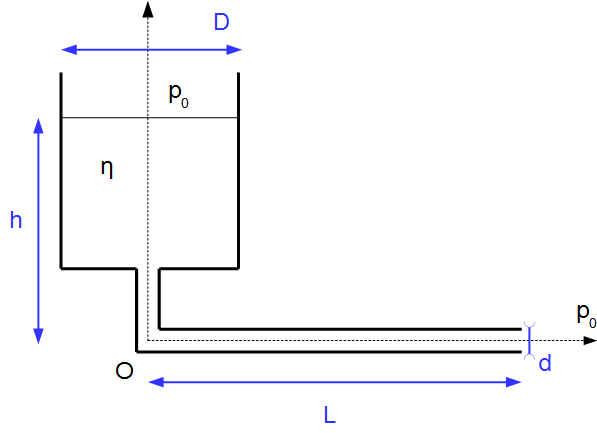
\includegraphics[scale = 0.4]{visco_poise.png}
	\caption{Schéma du problème} 
	\label{fig:visco_poise}
\end{center}
\end{figure}

\textcolor{red}{Fluide incompressible, donc conservation du débit volumique dans tout le système :}
le débit dans la citerne (notamment en haut) est égal au débit en sortie de conduite. 

On fait l'hypothèse d'un régime stationnaire, de sorte que dans la conduite, le débit volume est donné par la formule de Poiseuille :
\begin{equation}
	q_v = \frac{\pi d^4}{128\eta}\frac{p(O) -p_0}{L},
\end{equation}
la pression au point O étant une inconnue à déterminer.

Dans la citerne, le débit volumique à l'interface air/eau s'écrit :
\begin{equation}
	q_v = \iint_{\text{section citerne}}\bold{v}\cdot d\bold{\mathcal{S}} = -\pi\frac{D^2}{4}\frac{dh}{dt},
\end{equation}
car $\bold{v} = -dh/dt \bold{e}_z$ avec $h$ désignant la hauteur d'eau à partir du point O.

On a donc, par conservation du débit :
\begin{equation}
	-\pi\frac{D^2}{4}\frac{dh}{dt} = \frac{\pi d^4}{128\eta}\frac{p(O) -p_0}{L}.
\end{equation}

Il reste à déterminer $p(O)$. On supposant un écoulement stationnaire (la surface libre de l'eau contenue dans la citerne doit être grande devant la section de l'orifice de la conduite) et en négligeant la viscosité dans la citerne, l'équation de N.S. devient
\begin{equation}
 	0 = \rho \bold{g} - \textbf{grad}\;p + \eta\Delta{\bold{v}},
\end{equation}
d'où $p(z) = p_0 + \rho g(h-z)$.\\

Ainsi $p(O) = p_0 + \rho g h$, d'où
\begin{equation}
	-\pi\frac{D^2}{4}\frac{dh}{dt} = \frac{\pi d^4}{128\eta}\frac{\rho g h}{L}.
\end{equation}
Cette équation est une équation différentielle d'ordre 1 à coefficients constants et sans second membre, de sorte que

\begin{equation}
	h(t) = h_0 \text{exp}\;\left(-\frac{t}{\tau}\right),
\end{equation}
où $\tau = 32 \nu D^2 L/(g d^4)$.\\

\textcolor{red}{Application numérique :}
$h(t = 0) = 5$ cm, $h(t = 4500s) = 2.5$ cm, $D = 5$ cm, $d = 1$ mm, $L = 40$ cm et $g = 9.8 m/s^2$. 

\begin{equation}
	\text{ln}(h) = \text{ln}(h_0) - \frac{t}{\tau},
\end{equation} 
d'où
\begin{equation}
	\displaystyle{\nu = \frac{g d^4}{32D^2L}\frac{t}{\text{ln}\;\frac{h_0}{h}}}
\end{equation}

A.N. $\nu \sim 2.10^{-6} m^2/s$.

\section{Conclusion}

Rappelons les points importants : une portion de fluide exerce sur une autre, à travers la surface qui les sépare, une force de frottement tangentielle à la surface, proportionnelle au gradient de vitesse. La viscosité est la grandeur caractéristique de cette force. Ce phénomène s'apparente à un transport de quantité de mouvement par diffusion, visant à réduire l'ampleur du gradient de vitesse (tentative de retour à l'homogénéité des grandeurs intensives). Les forces de viscosités sont non conservatives et par conséquent dissipatives. Au bout d'un certain temps, le fluide retrouve son état de repos s'il n'est pas alimenté en énergie par une source extérieure. Cette dissipation se fait sous forme de chaleur (transfert d'énergie à l'échelle microscopique).

Un écoulement visqueux est solution de l'équation de Navier Stokes, qu'il est possible de simplifier en tenant compte de paramètres sans dimension. Le nombre de Reynolds, un de ces paramètres, permet de quantifier l'importance du terme d'advection par rapport à celle du terme de viscosité (diffusion). En présence d'un faible nombre de Reynolds, les phénomènes visqueux jouent un rôle important et l'écoulement conserve une structure ordonnée : l'écoulement est dit rampant. Si le Reynolds est élevé ($Re > 2000$), les phénomènes d'advection prennent le dessus. Leur grande non-linéarité est potentiellement source d'instabilité : le fluide peut se déstructurer, des tourbillons apparaissent sur un continuum d'échelles de longueur et l'écoulement est dit turbulent. 

Dans des systèmes de grande taille, les phénomènes de viscosité perdent de leur importance au fur et à mesure que l'on s'éloigne des bords. En dehors d'une zone située à l'interface paroi/fluide appelée couche limite, d'épaisseur inversement proportionnelle à la racine carrée du nombre de Reynolds, les phénomènes de viscosité peuvent être négligés : c'est l'approximation de l'écoulement parfait, qui fera l'objet de la leçon suivante.
\end{document}